\documentclass[11pt]{article}
\usepackage{listings}
\usepackage{tikz}
\usepackage{enumerate}
\usetikzlibrary{arrows,automata,shapes}
\tikzstyle{block} = [rectangle, draw, fill=blue!20, 
    text width=5em, text centered, rounded corners, minimum height=2em]
\tikzstyle{bt} = [rectangle, draw, fill=blue!20, 
    text width=4em, text centered, rounded corners, minimum height=2em]


\newtheorem{defn}{Definition}
\newtheorem{crit}{Criterion}

\newcommand{\handout}[5]{
  \noindent
  \begin{center}
  \framebox{
    \vbox{
      \hbox to 5.78in { {\bf Software Testing, Quality Assurance and Maintenance } \hfill #2 }
      \vspace{4mm}
      \hbox to 5.78in { {\Large \hfill #5  \hfill} }
      \vspace{2mm}
      \hbox to 5.78in { {\em #3 \hfill #4} }
    }
  }
  \end{center}
  \vspace*{4mm}
}

\newcommand{\lecture}[4]{\handout{#1}{#2}{#3}{#4}{Lecture #1}}
% 1-inch margins, from fullpage.sty by H.Partl, Version 2, Dec. 15, 1988.
\topmargin 0pt
\advance \topmargin by -\headheight
\advance \topmargin by -\headsep
\textheight 8.9in
\oddsidemargin 0pt
\evensidemargin \oddsidemargin
\marginparwidth 0.5in
\textwidth 6.5in

\parindent 0in
\parskip 1.5ex
%\renewcommand{\baselinestretch}{1.25}

% http://gurmeet.net/2008/09/20/latex-tips-n-tricks-for-conference-papers/
\newcommand{\squishlist}{
 \begin{list}{$\bullet$}
  { \setlength{\itemsep}{0pt}
     \setlength{\parsep}{3pt}
     \setlength{\topsep}{3pt}
     \setlength{\partopsep}{0pt}
     \setlength{\leftmargin}{1.5em}
     \setlength{\labelwidth}{1em}
     \setlength{\labelsep}{0.5em} } }
\newcommand{\squishlisttwo}{
 \begin{list}{$\bullet$}
  { \setlength{\itemsep}{0pt}
     \setlength{\parsep}{0pt}
    \setlength{\topsep}{0pt}
    \setlength{\partopsep}{0pt}
    \setlength{\leftmargin}{2em}
    \setlength{\labelwidth}{1.5em}
    \setlength{\labelsep}{0.5em} } }
\newcommand{\squishend}{
  \end{list}  }

\lstset{numbers=left,numberstyle=\scriptsize,basicstyle=\ttfamily}
\begin{document}

\lecture{9 --- January 23, 2015}{Winter 2015}{Patrick Lam}{version 1}

\section*{Graph Coverage for Source Code}

So far, we've seen a number of coverage criteria for
graphs, but I've been vague about how to actually
construct graphs. For the most part, it's fairly obvious.

%Let's see formal definitions. Remember that we first defined
%the structural criteria: NC, EC, EPC, PPC, SPC, CPC.
%{\sf (Why are ADC, AUC, ADUPC, CRTC, SRTC inapplicable?)}\\[1em]

\subsection*{Structural Graph Coverage for Source Code}

Fundamental graph for source code: \emph{Control-Flow Graph} (CFG).

\begin{itemize}
\item CFG nodes: zero or more statements;
\item CFG edges: an edge $(s_1, s_2)$ indicates that $s_1$ may
  be followed by $s_2$ in an execution.
\end{itemize}

\paragraph{Basic Blocks.} We can simplify a CFG by grouping together
statements which always execute together (in sequential programs):

\begin{tabular}{ll}
\begin{minipage}{.4\textwidth}
\begin{lstlisting}
    x = 5
    z = 2
q0: if (z < 17) goto q1
    z = z + 1
    print (x)
    goto q0
q1: nop
\end{lstlisting}
\end{minipage} &
\begin{minipage}{.5\textwidth}
\begin{center}
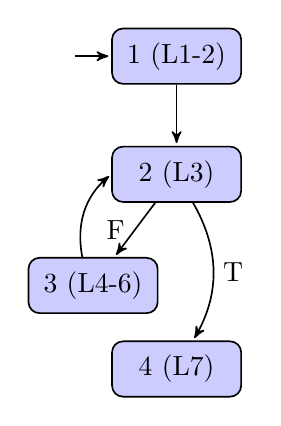
\begin{tikzpicture}[->,>=stealth',shorten >=1pt,auto,node distance=1.5cm,
                    semithick,initial text=]

  \node[initial,bt]   (1)                     {1 (L1-2)};
  \node[bt]           (2) [below of=1] {2 (L3)};
  \node[bt]           (3) [below left of=2,yshift=-1em] {3 (L4-6)};
  \node[bt]           (4) [below right of=3] {4 (L7)};

  \path (1) edge node {} (2)
        (2) edge node[left] {F} (3)
            edge [bend left] node {T} (4)
        (3) edge [bend left] node {} (2.west);
\end{tikzpicture}
\end{center}

\end{minipage}
\end{tabular}

We use the following definition:
\begin{defn}
A basic block has one entry point and one exit point.
\end{defn}
Note that a basic block may have multiple successors. However, there 
may not be any jumps into the middle of a basic block (which is
why statement {\tt l0} has its own basic block.)

\subsection*{Some Examples} We'll now see how to construct
control-flow graph fragments for various program constructs.

{\bf if statements:} The book puts the conditions
(and hence uses) on the control-flow edges, rather than in the 
{\tt if} node. I prefer putting the condition in the node.

\begin{tabular}{ll|ll}
\begin{minipage}{.15\textwidth}
\begin{lstlisting}
if (z < 17)
  print (x);
else
  print (y);
\end{lstlisting}
\end{minipage} &
\begin{minipage}{.3\textwidth}
\begin{center}
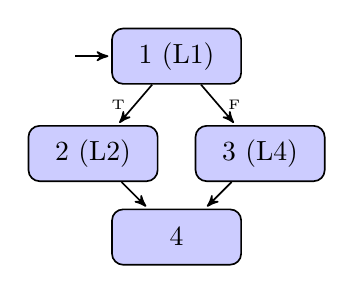
\begin{tikzpicture}[->,>=stealth',shorten >=1pt,auto,node distance=1.5cm,
                    semithick,initial text=]

  \node[initial,bt]   (1)                     {1 (L1)};
  \node[bt]           (2) [below left of=1,yshift=-0.5em] {2 (L2)};
  \node[bt]           (3) [below right of=1,yshift=-0.5em] {3 (L4)};
  \node[bt]           (4) [below left of=3] {4};

  \path (1) edge node[left] {\tiny T} (2)
        (1) edge node[right] {\tiny F} (3)
        (2) edge node {} (4)
        (3) edge node {} (4);
\end{tikzpicture}
\end{center}
\end{minipage}&
\begin{minipage}{.3\textwidth}
\begin{center}
\begin{tikzpicture}[->,>=stealth',shorten >=1pt,auto,node distance=1.5cm,
                    semithick,initial text=]

  \node[initial,bt]   (1)                     {1 (L1)};
  \node[bt]           (2) [below left of=1,yshift=-0.5em] {2 (L2)};
  \node[bt]           (4) [below left of=3] {3};

  \path (1) edge node[left] {\tiny T} (2)
        (1) edge node[right] {\tiny F} (4)
        (2) edge node {} (4);
\end{tikzpicture}
\end{center}
\end{minipage}
& \begin{minipage}{.1\textwidth}
\begin{lstlisting}
if (z < 17)
  print(x);
\end{lstlisting}
\end{minipage}
\end{tabular}

Short-circuit {\tt if} evaluation is more complicated; I recommend working it out yourself.

(Recall that node coverage does not imply edge coverage.)


{\bf case / switch statements:} 

\begin{tabular}{ll}
\begin{minipage}{.45\textwidth}
\begin{lstlisting}
switch (n) {
  case `I': ...; break;
  case `J': ...; /* fall thru */
  case `K': ...; break;
}
// ...
\end{lstlisting}
\end{minipage} &
\begin{minipage}{.4\textwidth}
\begin{center}
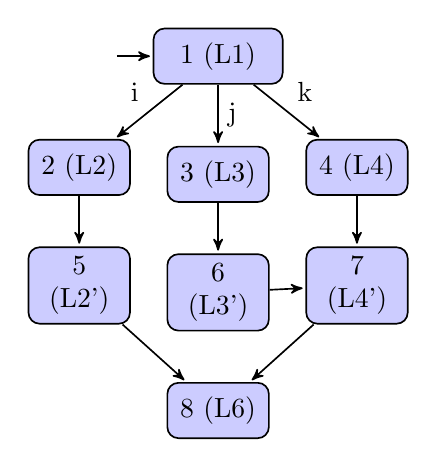
\begin{tikzpicture}[->,>=stealth',shorten >=1pt,auto,node distance=1.5cm,
                    semithick,initial text=]

  \node[initial,bt]   (1)                     {1 (L1)};
  \node[bt, text width=3em]           (2) [below left of=1,xshift=-2em,yshift=-1em]  {2 (L2)};
  \node[bt, text width=3em]           (3) [below of=1]   {3 (L3)};
  \node[bt, text width=3em]           (4) [below right of=1,xshift=2em,yshift=-1em]   {4 (L4)};
  \node[bt, text width=3em]           (5) [below of=2]  {5 (L2')};
  \node[bt, text width=3em]           (6) [below of=3]  {6 (L3')};
  \node[bt, text width=3em]           (7) [below of=4]  {7 (L4')};
  \node[bt, text width=3em]           (8) [below of=6]  {8 (L6)};

  \path 
  (1) edge node[left,yshift=0.7em] {i} (2)
  (1) edge node {j} (3)
  (1) edge node {k} (4)
  (2) edge node {} (5)
  (3) edge node {} (6)
  (4) edge node {} (7)
  (6) edge node {} (7)
  (5) edge node {} (8)
  (7) edge node {} (8);
\end{tikzpicture}
\end{center}
\end{minipage}
\end{tabular}

{\bf while statements:}

\begin{tabular}{ll}
\begin{minipage}{.2\textwidth}
\begin{lstlisting}
x = 0; y = 20;
while (x < y) {
  x ++; y --;
}
\end{lstlisting}
\end{minipage} &
\begin{minipage}{.4\textwidth}
\begin{center}
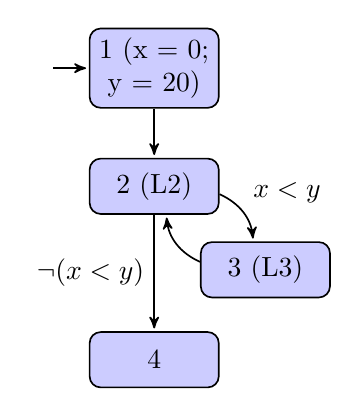
\begin{tikzpicture}[->,>=stealth',shorten >=1pt,auto,node distance=1.5cm,
                    semithick,initial text=]

  \node[initial,bt]   (1)                     {1 (x = 0; y = 20)};
  \node[bt]           (2) [below of=1]        {2 (L2)};
  \node[bt]           (3) [below right of=2,xshift=1em]  {3 (L3)};
  \node[bt]           (4) [below of=2,yshift=-2em]   {4};

  \path (1) edge node {} (2)
  (2) edge [bend left] node {$x < y$} (3)
  (3) edge [bend left] node {} (2)
  (2) edge node[left] {$\neg (x < y)$} (4);
\end{tikzpicture}
\end{center}
\end{minipage}
\end{tabular}

Note that arbitrarily complicated structures may occur inside
the loop body.

{\bf for statements:} 

\begin{tabular}{ll}
\begin{minipage}{.5\textwidth}
\begin{lstlisting}
for (int i = 0; i < 57; i++) {
  if (i % 3 == 0) {
    print (i);
  }
}
\end{lstlisting}
\end{minipage} & \begin{minipage}{.4\textwidth}
  (an exercise for the reader!)
\end{minipage}
\end{tabular}

\newpage
This example uses Java's enhanced for loops, which iterates over all of the elements
in the {\tt widgetList}:

\begin{lstlisting}[basicstyle=\scriptsize \ttfamily]
for (Widget w : widgetList) {
  decorate(w);
}
// ...
\end{lstlisting}

I will accept the simplified CFG or the more useful one on the right:

\begin{tabular}{ll}
\begin{minipage}{.4\textwidth}
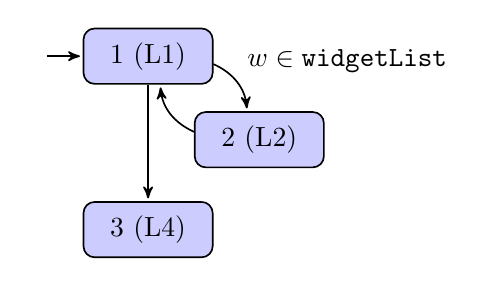
\begin{tikzpicture}[->,>=stealth',shorten >=1pt,auto,node distance=1.5cm,
                    semithick,initial text=]

  \node[initial,bt]   (1)                     {1 (L1)};
  \node[bt]           (3) [below right of=1,xshift=1em]  {2 (L2)};
  \node[bt]           (4) [below of=1,yshift=-2em]   {3 (L4)};

  \path 
  (1) edge [bend left] node {$w \in \mbox{\tt widgetList}$} (3)
  (3) edge [bend left] node {} (1)
  (1) edge node[left] {} (4);
\end{tikzpicture}
\end{minipage} &
\begin{minipage}{.5\textwidth}
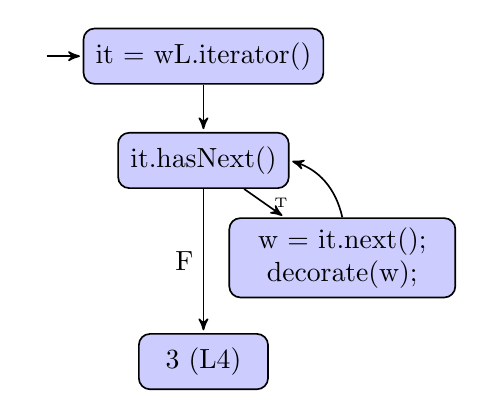
\begin{tikzpicture}[->,>=stealth',shorten >=1pt,auto,node distance=1.5cm,
                    semithick,initial text=]

  \node[initial,bt,text width=8em]   (1)                     {it = wL.iterator()};
  \node[bt,text width=5.5em]            (2) [below of=1,yshift=.5em] {it.hasNext()};
  \node[bt,text width=7.5em]           (3) [below right of=2,xshift=2em,yshift=-.5em]  {w = it.next(); decorate(w);};
  \node[bt]           (4) [below of=2,yshift=-3em]   {3 (L4)};

  \path (1) edge node {} (2)
        (2) edge node[right] {\tiny T} (3)
        (3.north) edge [bend right] node {} (2.east)
        (2) edge node[left] {F} (4);
%  (1) edge [bend left] node {$w \in \mbox{\tt widgetList}$} (3)
%  (3) edge [bend left] node {} (1)
%  (1) edge node[left] {} (4);
\end{tikzpicture}
\end{minipage}
\end{tabular}

All of these graphs admit the notions of node coverage (statement
coverage, basic block coverage) and edge coverage (branch coverage).

\paragraph{Larger example.} You can draw a 7-node CFG for this program:

\begin{lstlisting}[basicstyle=\scriptsize\ttfamily]
  /** Binary search for target in sorted subarray a[low..high] */
  int binary_search(int[] a, int low, int high, int target) {
    while (low <= high) {
      int middle = low + (high-low)/2;
      if (target < a[middle)
        high = middle - 1;
      else if (target > a[middle])
        low = middle + 1;
      else
        return middle;
    }
    return -1; /* not found in a[low..high] */
  }
\end{lstlisting}

\vspace*{-2em}
\begin{center}
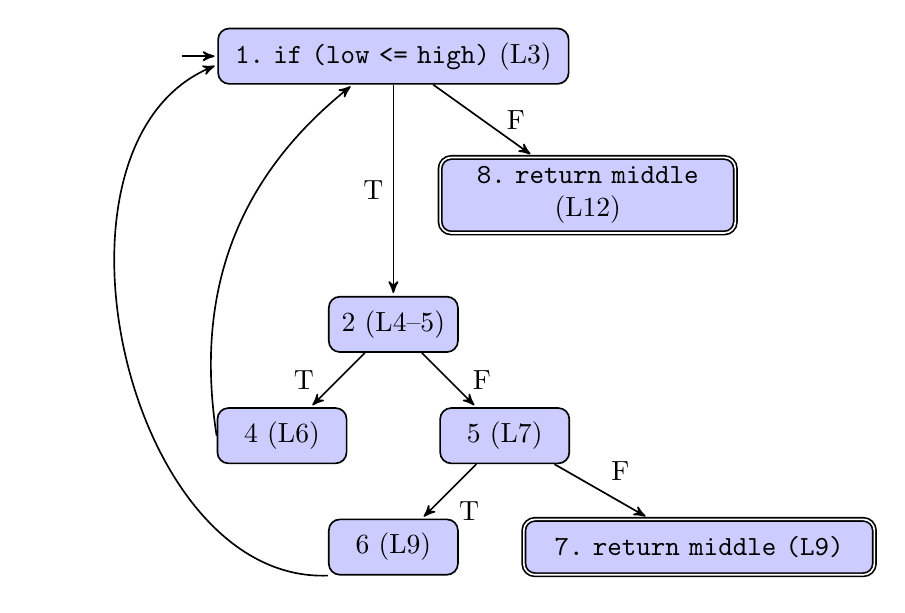
\begin{tikzpicture}[->,>=stealth',shorten >=1pt,auto,node distance=2cm,
                    semithick,initial text=]
  \node[initial,bt,text width=12em]   (1)                     {\verb+1. if (low <= high)+ (L3)};
  \node[bt, accepting,text width=10em]          (8) [below right of=1,yshift=-1em,xshift=3em]  {\verb+8. return middle+ (L12)};
  \node[bt]           (2) [below of=1, yshift=-4em]  {2 (L4--5)};
  \node[bt]           (4) [below left of=2] {4 (L6)};
  \node[bt]           (5) [below right of=2] {5 (L7)};
  \node[bt]           (6) [below left of=5] {6 (L9)};
  \node[bt,text width=12em,accepting,xshift=3em]           (7) [below right of=5] {\verb+7. return middle (L9)+};

  \path (1) edge node[left] {T} (2)
  (1) edge node[right,xshift=.5em] {F} (8)
  (2) edge node[left,xshift=-.5em] {T} (4)
  (2) edge node[right,xshift=.5em]{F} (5)
  (4.west) edge [bend left] (1)
  (5) edge node {T} (6)
  (5) edge node {F} (7)
  (6.south west) edge [bend left=80] (1);
\end{tikzpicture}
\end{center}

\newpage
\section*{Exercises}
Here are more exercise programs that you can draw CFGs for.
\begin{lstlisting}[basicstyle=\scriptsize\ttfamily]
/* effects: if x==null, throw NullPointerException
            otherwise, return number of elements in x that are odd, positive or both. */
int oddOrPos(int[] x) {
  int count = 0;
  for (int i = 0; i < x.length; i++) {
    if (x[i]%2 == 1 || x[i] > 0) {
      count++;
    }
  }
  return count;
}

// example test case: input: x=[-3, -2, 0, 1, 4]; output: 3  
\end{lstlisting}

Next, we have a really poorly-designed API (I'd give it a D at most,
maybe an F) because it's impossible to succinctly describe what it
does. {\bf Do not design functions with interfaces like this.} But we
can still draw a CFG, no matter how bad the code is.
\begin{lstlisting}[basicstyle=\scriptsize\ttfamily]
  /** Returns the mean of the first maxSize numbers in the array,
      if they are between min and max. Otherwise, skip the numbers. */
  double computeMean(int[] value, int maxSize, int min, int max) {
    int i, ti, tv, sum;

    i = 0; ti = 0; tv = 0; sum = 0;
    while (ti < maxSize) {
      ti++;
      if (value[i] >= min && value[i] <= max) {
        tv++;
        sum += value[i];
      }
      i++;
    }
    if (tv > 0)
      return (double)sum/tv;
    else
      throw new IllegalArgumentException();
  }
\end{lstlisting}

\end{document}
